\documentclass[a4paper,oneside,frenchb,12pt]{article}
\usepackage{amsmath}
\usepackage[mathletters]{ucs}
\usepackage[utf8x]{inputenc}
\usepackage[T1]{fontenc}
\usepackage[breaklinks=true,unicode=true]{hyperref}
\usepackage{geometry}
\usepackage{fourier}
\setlength{\parindent}{0pt}
\setlength{\parskip}{6pt plus 2pt minus 1pt}
\setcounter{secnumdepth}{0}
\usepackage{amsmath}
\usepackage{babel}
\usepackage{textcomp}
\usepackage{graphicx}
\usepackage{url}
\usepackage{hyperref}

\hypersetup{
    colorlinks,%
    citecolor=black,%
    filecolor=black,%
    linkcolor=black,%
    urlcolor=black
}
%\urlstyle{sf}
\pagestyle{plain}
\geometry{ hmargin=1.5cm, vmargin=1.5cm }
\begin{document}

\section{Manuel utilisateur}

\subsection{Introduction}

Tout d'abord, nous vous remercions d'avoir choisi notre logiciel
SynthPro. Les BackSynth Boys ont travaillé dur pour produire ce
logiciel sonore qui saura vous convaincre de sa haute qualité.

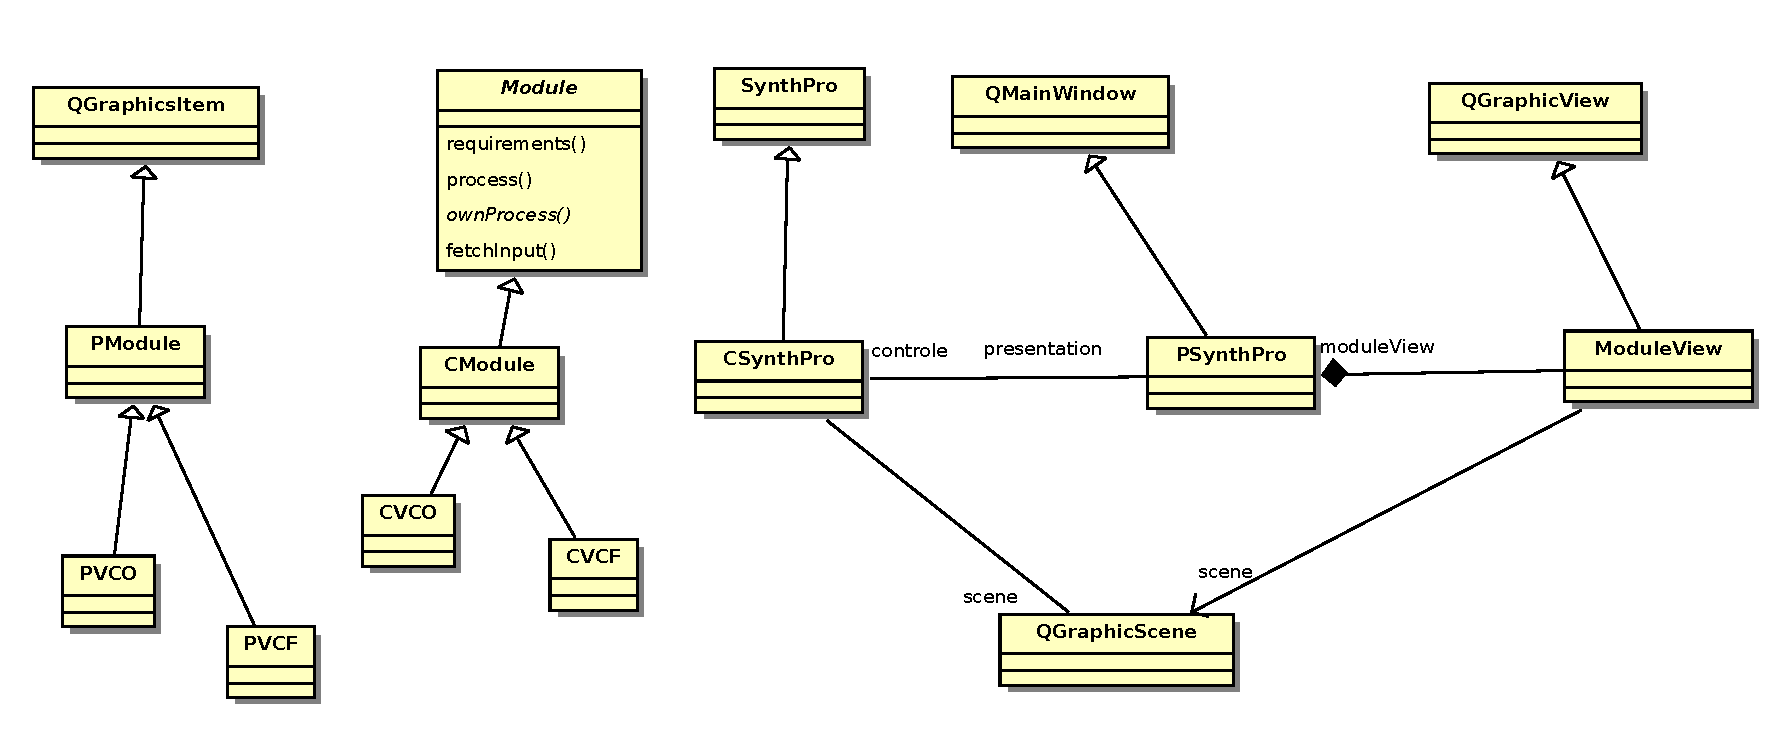
\includegraphics[width=18cm]{../img/pac.pdf}


\subsection{Présentation générale}

SynthPro est un logiciel de synthèse sonore dont le but est de
simuler les différents modules utilisés par les synthétiseurs
analogiques dits à synthèse soustractive.

Ce logiciel est entièrement modulable. Vous pouvez placer les
modules mis à votre disposition, les lier entre eux et entendre le
résultat du montage en temps-réel. Il ne reste plus qu'à laisser
votre créativité faire le reste.

\subsection{Utilisation du logiciel}

Lorsque vous lancez le logiciel, vous verrez apparaitre son
interface :

\begin{itemize}
\item
  Les menus en haut
\item
  La barre d'outil
\item
  Les modules disponibles classés selon leur type, à gauche
\item
  Un grand espace vide que vous allez pouvoir remplir !
\end{itemize}
\subsubsection{Les menus}

Ils sont composés de deux options : File et Help, chacun possédant
des sous-menus.

File

\begin{itemize}
\item
  New : Vous permet de recommencer un nouveau montage, après
  confirmation de votre part d'effacer le montage courant.
\item
  Play/Pause : Permet de stopper ou de rétablir la lecture du
  montage. Stopper la lecture revient à couper le son et stopper
  toute la gestion des modules en temps-reel.
\item
  Exit : Provoque la sortie de l'application.
\end{itemize}
Help

\begin{itemize}
\item
  About : Donne des informations relatives au logiciel et ses
  développeurs.
\item
  About Qt : Donne des informations relatives au framework utilisé
  pour le développement de ce logiciel.
\item
  Exit
\end{itemize}
\subsubsection{La barre d'outil}

Les trois actions disponibles dans la barre d'outil sont identiques
à ce que l'on peut trouver dans le menu File, ci dessus : New,
Exit, et Play/Pause.

\subsubsection{Les modules classés}

Les modules ont été classés en trois catégories :

\begin{itemize}
\item
  Les modules d'entrée (Input modules)
\item
  Les modules de traitements (Modules)
\item
  Les modules de sortie (Output modules)
\end{itemize}
Les modules d'entrée représentent les modules qui peuvent créer des
signaux à partir de rien. Ce sont les composants de base d'un
montage et ne disposent pas d'entrée.

Les modules de traitements sont intermédiaires : ils prennent un
signal, le modifient et le renvoient sur leur sortie.

Enfin, les modules de sortie sont mis en fin de chaîne : ils
acceptent une entrée, mais ne renvoient rien car ils n'ont pas de
sortie.

L'interface vous sera présentée ultérieurement.

\subsection{Présentation générale de la modularité}

SynthPro est un logiciel modulaire : chaque module est une
``brique'' qu'il est possible de placer un nombre infini de fois
sur l'interface, afin de construire votre propre montage sonore.

Un module dispose de plusieurs caractéristiques :

\begin{itemize}
\item
  Une fonction
\item
  Une ou plusieurs ports d'entrées
\item
  Une ou plusieurs ports de sorties
\item
  Des paramètres
\end{itemize}
La fonction du filtre est en général clairement définie par son
nom. Ainsi, le module filtre va\ldots{} filtrer ce qu'on lui
donne.

Les ports d'entrée servent à fournir du signal au module. Ainsi, un
filtre aura forcément besoin de données à traiter, afin qu'il
puisse accomplir sa fonction.

Les ports de sortie servent à renvoyer le travail produit à un
autre module, ou plutôt, à l'une de ses entrées. Ainsi, une chaîne
entière sonore peut être fabriquée en liant les sorties des modules
aux entrées des autres.

Les paramètres des modules peuvent apparaitre sous plusieurs formes
: potentiomètres ou slider à coulisser. Ces paramètres dépendent
entièrement du module. Ainsi, un module Mixer pourra changer le
volume de chacune de ses entrées grâce au paramètre Gain qui leur
est attribué.

Les modules peuvent être reliés par des cables virtuels, qui
représenteraient des cables électriques dans
``le monde réel''\ldots{} Mais les nôtres sont infaillibles.

\subsection{Description des modules.}

TODO : placer ici la description des modules (depuis autre
fichier).

\subsection{Utilisation pratique du logiciel}

Il est maintenant temps de commencer à créer des montages sonores
dignes de ce nom. Le grand espace vide à droite de la liste des
modules va servir à cela. La première étape consiste à prendre un
module et le placer dans la zone de montage. Pour cela, cliquez sur
le module désiré grâce au bouton gauche de la souris et, sans le
relâcher, déplacer votre curseur au milieu de la zone de montage.
Relâchez le bouton. Le module va alors être créé.

Essayez de le faire avec le module d'entrée VCO. Vous pouvez voir
les différentes types d'onde qu'il peut produire. Comme il s'agit
d'un module d'entrée, il ne dispose pas d'entrées, car il produit
lui-même un flux de données. Il dispose par contre d'une sortie
Out. On peut également voir grâce au potentiomètre K que le VCO
produit une onde à 261 Hz, soit un DO de l'octave 4.

Mais pour l'instant, aucun son n'est entendu. Pour cela, il faut
une sortie son : placez à droite du module présent un module Audio
Output. Celui-ci est un module de sortie, il n'a donc pas de
sorties, mais une entrée. Il faut donc relier celle-ci à la sortie
du VCO. Pour cela, cliquez simplement sur l'entrée et, sans
relâcher le bouton gauche de la souris, déplacer votre curseur vers
la sortie du VCO. Un câble vient d'apparaitre. Vous pouvez voir les
ports sur lesquels vous pouvez accrocher le câble devenir verts.
Les emplacements non accessibles sont affichés en rouge. Lâchez
alors le bouton pour créer la connexion entre les deux ports. Le
son produit par le VCO est maintenant reproduit par vos
haut-parleurs !

Il vous est possible de relier tout port de sortie vers une entrée,
et inversement. Pour débrancher un câble, cliquez sur une de ses
extrémités et relâchez le bouton de la souris lorsque le cable
survole une zone non-interactive, comme le fond de la zone de
montage. Il est vous également possible de rebrancher le cable sur
une autre entrée si besoin est.

Vous pouvez ainsi ajouter tous les modules que vous désirez et les
relier entre eux. Si vous souhaitez retirer un module, cliquez
simplement sur la croix en haut à gauche de chacun d'eux.

Vous avez maintenant toutes les clefs en main pour obtenir des sons
prodigieux !

\subsection{Quelques montages type}

TODO

\subsection{Conclusion}

Nous espérons que ce produit vous apportera entière satisfaction.
N'hésitez pas à nous faire part de vos suggestions afin que nous
continuons d'améliorer notre produit !

Cordialement, Les Backsynth Boys.

\end{document}

